
\newpage
\subsection{SVI (Serveur vocal interactif)}

\textit{
«Un serveur vocal interactif (en anglais Interactive Voice Response) est un système informatique permettant aux utilisateurs d'accéder à la base de données d'une société et d'émettre diverses demandes de service, au moyen d'un téléphone fixe, mobile ou logiciel. Les serveurs vocaux interactifs entrent plus généralement dans la catégorie des systèmes de dialogue.}\\

\textit{«La nouvelle génération de serveurs vocaux interactifs permet de traiter et de publier tous types de médias (sons, images, vidéos) et de données (base de données, fichiers textes, xml, pages web). Le VoiceXML, langage reconnu par le W3C, standardise les développements et redonne une forte impulsion à ces systèmes.»}\\ 

\rightline{-- Wikipédia}

\subsubsection{Paiement par SVI}
Le paiement par le SVI permet le déroulement de la cinématique de paiement classique, mais sur le canal vocal. Avec autant de garanties de sécurité pour le commerçant. Tous les paiements à distance devant respecter la norme PCI/DSS, l’interface vocale permet donc de proposer un paiement sécurisé sur ce canal.\\

Les principaux objectifs de l’application pour le commerçant :
\begin{itemize}
\item Réduire les coûts de traitement des paiements
\item Sécuriser les paiements
\item Proposer un nouveau canal de paiement et élargir la clientèle\\
\end{itemize}

Avec deux cas d’utilisation possibles:\footnote{\url{http://www.sips-atos.com/fr/63/L-offre-en-detail/Multicanal/Serveur-vocal-interactif.html}} 

\begin{figure}[!htbp]
  \centering
    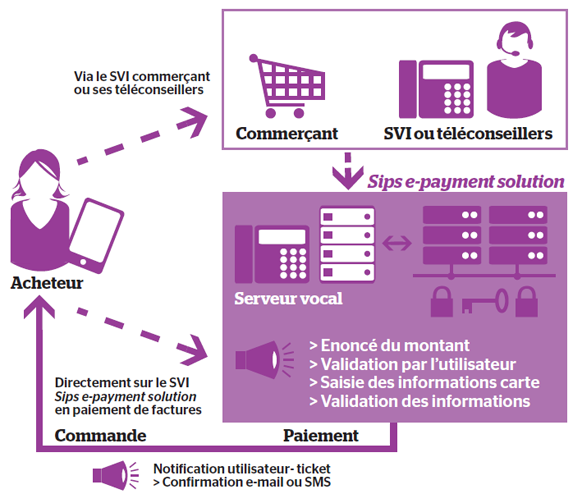
\includegraphics[scale=0.4]{images/SVI}
  \caption{cas d’utilisation de SVI}
\end{figure}


\subsubsection{Le SVI de paiement de factures}

La solution de paiement de factures via le SVI permet à un commerçant d’émettre des factures qui seront payables, entre autres, via un téléphone sur un SVI sécurisé. Ce qui peut représenter un canal complémentaire de paiement pour un commerçant, et éviter le traitement de chèques par exemple.\\

Cette offre permet à des fournisseurs de services d’offrir à leurs clients finaux un nouveau moyen de paiement à distance de leurs factures grâce à un SVI de paiement sécurisé. L’interconnexion avec les fournisseurs de services permet d’identifier la facture à régler et le client final est invité à effectuer le paiement de celle-ci en saisissant, en parfaite autonomie, les informations de sa carte de paiement.

\subsubsection{Le routage par le centre d'appels} 

Le SVI permet à un téléconseiller marchand de transférer son client vers le SVI au moment de la finalisation de la transaction en cours. Le client, transféré sur ce SVI, est informé de la transaction pour laquelle le paiement va être réalisé et est ensuite invité à finaliser cette transaction en saisissant les informations de sa carte de paiement. La saisie de ces informations est réalisée par le possesseur de la carte lui-même, elles ne sont donc pas divulguées à une tierce personne.\\

Et ainsi :
\begin{itemize}
\item Gagner du temps d’occupation des téléopérateurs et donc de réduire les coûts de traitement des appels
\item Sécuriser le processus et éviter aux téléopérateurs d’avoir connaissance des informations carte du client
\item Proposer de nouveaux services qui feront l’objet d’un paiement via ce canal\\
\end{itemize}

Le paiement via le SVI permet donc d’élargir le champ d’action commercial, de proposer du paiement en toute sérénité, et surtout de diminuer les coûts de traitement des appels ou d’encaissement. 



\subsubsection{SVI d'UINT}

Pour l'utilisation du système SVI d'UINT, nous avons conçu trois modes d'utilisations à choisir par les utilisateurs:\\

\textbf{Mode 1: Utilisation classique}\\
L'utilisateur utilise sa carte acoustique et le code PIN avec son téléphone, le statut est visualisé sur la page Web.

\begin{figure}[!htbp]
  \centering
    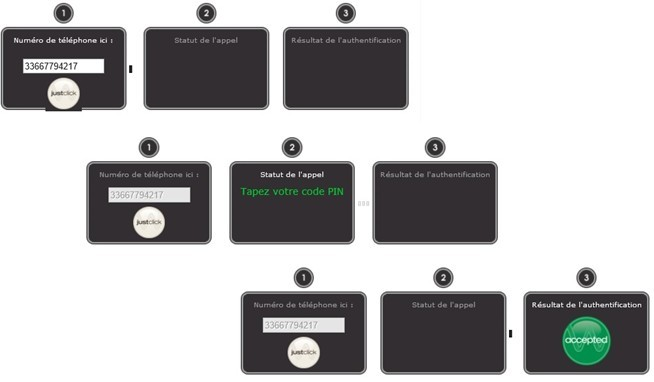
\includegraphics[scale=1]{images/mode1}
  \caption{Mode 1 de cas d’utilisation de SVI}
\end{figure}

\newpage
\textbf{Mode 2: Utilisation classique + Code dynamique}\\
Le deuxième mode est similaire au premier, mais il ajoute une étape de vérification par un mot de passe dynamique envoyé par SMS à l'utilisateur.

\begin{figure}[!htbp]
  \centering
    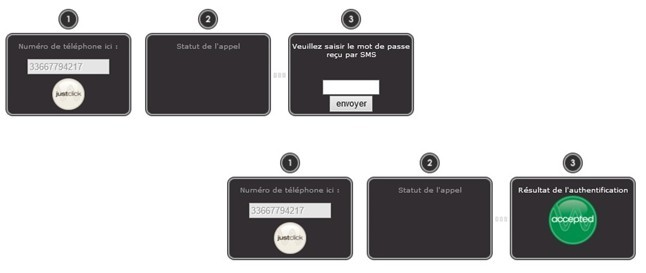
\includegraphics[scale=1]{images/mode2}
  \caption{Mode 2 de cas d’utilisation de SVI}
\end{figure}
\newpage
%\begin{wrapfigure}[]{r}{70mm}
%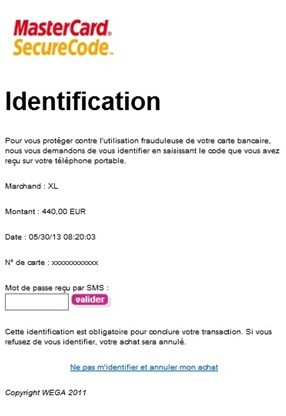
\includegraphics[scale=0.8]{images/mode3}
%\caption{Mode 3 de cas d’utilisation de SVI}
%\end{wrapfigure}

\textbf{Mode 3: Code dynamique}\\
Le troisième mode est destiné aux ceux qui ne peuvent pas utiliser la carte acoustique, l'authentification est réalisée par un code dynamique seulement, qui est envoyé par SMS à l'utilisateur.% c'est comme l'utilisation d'une carte bancaire en ligne qui existe sur beaucoup de site commerçant aujourd'hui .

\begin{figure}[!htbp]
  \centering
    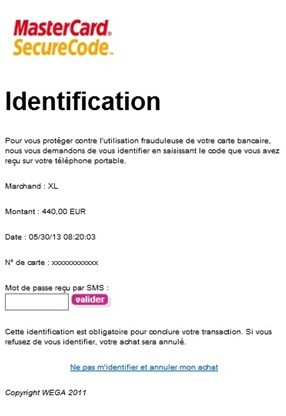
\includegraphics[scale=1]{images/mode3}
  \caption{Mode 3 de cas d’utilisation de SVI}
\end{figure}

Un schéma figurant la procédure d'utilisation du SVI et son principe est disponible en Annexe \ref{svi}.

